\section{What survives}
\label{sec:survives}

The MoE-matched comparison shrinks the niche dramatically. DG only
wins above $L^{*} = 368$ tokens, and the margin is thin: $1.4\times$
at $L{=}1024$, $2.4\times$ at $L{=}2048$. The five conditions that
must all hold are:
\begin{enumerate}[nosep]
  \item Output length $\geq 1000$ tokens (naturally long, not forced).
  \item Batch-1 by requirement (tenant isolation, interactivity, or
    serial chain structure).
  \item Completeness is validated against a schema.
  \item The quality floor exceeds what the AR model delivers.
  \item A \dgWeights\,GB resident footprint is acceptable.
\end{enumerate}

\paragraph{Concrete workloads.}

\textit{Serial investigation chains.} A security operations centre
receives an alert, looks up threat intelligence, cross-references
internal logs, and drills into the next layer. Each hop blocks on the
previous; concurrency is 1 by construction. DG's per-hop p50 is
$\sim$410\,ms against AR-30B's $\sim$130\,ms at natural record length
--- AR wins per hop. DG's advantage only emerges at chain depth
$D \geq 8$, where the cumulative output exceeds 1000 tokens.

\begin{figure}[t]
\centering
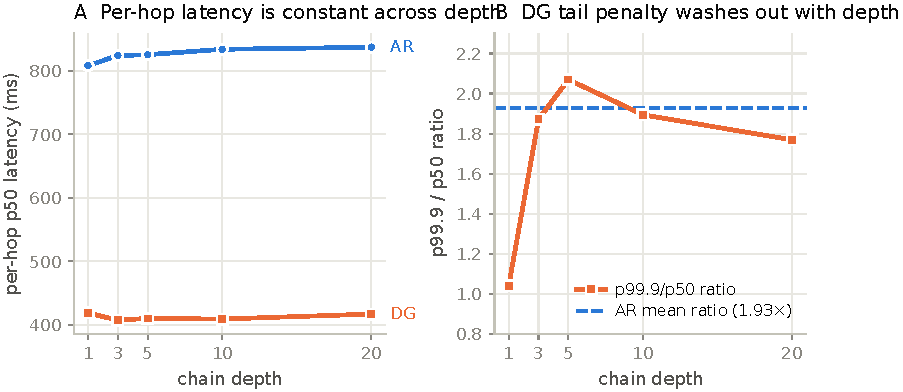
\includegraphics[width=\linewidth]{figures/fig10_usecase_chains.pdf}
\caption{Serial investigation chains (BGL, $n{=}300$, $K{=}8$).
\textbf{A:} per-hop p50 is constant across depth. \textbf{B:} DG's
p99.9/p50 ratio converges to AR's mean as depth increases.}
\label{fig:chains}
\end{figure}

\textit{Critical-alert preemption.} A FATAL log line arrives
mid-stream. DG's lower service time ($\sim$420\,ms) is available on
demand via priority preemption, but AR-30B is faster ($\sim$130\,ms
per event at natural length).

\textit{Autonomous driving.} One vehicle, one scene, one decision:
batch-1 by construction. Output is long (multi-object scene
description). The $K$ knob is a per-request quality slider with two
usable positions ($K{=}8$ and $K{=}4$). The completeness guarantee
holds only above the canvas length; below $L{=}128$ DG's schema
validity collapses (1.0\%, see Appendix~\ref{app:quality}).

\textit{Algorithmic trading.} A serial chain with a 1--5\,s market
reaction window. At 8 hops (L$\approx$1120), DG is $1.3\times$ faster
than AR-30B. At fewer hops, AR wins.

\textit{Wide-schema normalisation.} DG's joint-canvas denoising
treats all fields as one structured object. We measured schema widths
$F \in \{12, 25, 50, 100\}$: DG's latency advantage holds at
$1.8$--$3.0\times$ against the dense AR baselines, but has not been
measured against AR-30B MoE.

\begin{figure}[t]
\centering
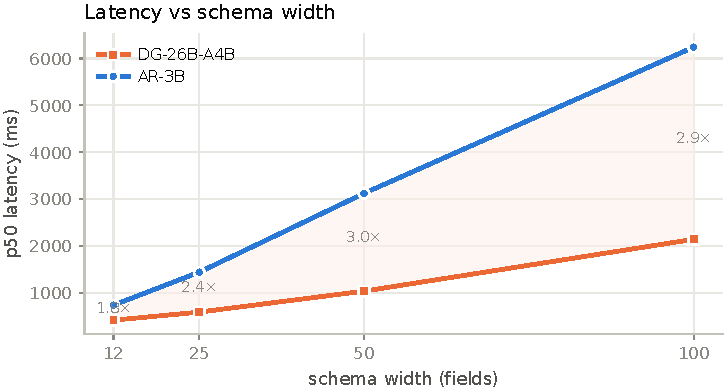
\includegraphics[width=0.85\linewidth]{figures/fig11_usecase_schema.pdf}
\caption{Latency vs schema width (BGL, $n{=}300$).}
\label{fig:schema}
\end{figure}

\paragraph{Where diffusion does not win.}

High-rate log streams ($\lambda \gg 2.6$ ev/s) favour AR's batching
by $45\times$ or more. Tail-sensitive single-stream workloads with
strict p99 SLAs are hurt by DG's $3.21\times$ max/median ratio. And
any workload that can batch favours AR regardless of output length.

\paragraph{Where diffusion fails.}

Six hypotheses about diffusion's structural advantages were tested and
refuted (Appendix~\ref{app:refuted}). The most instructive failures:

\begin{itemize}[nosep]
\item \textbf{Input perturbation robustness:} bidirectional attention
  propagates input noise in both directions. DG degraded more than AR
  in \emph{all 10} perturbation categories, by up to $8.2\times$ the AR
  drop.
\item \textbf{Infilling:} DG's joint denoising should preserve suffix
  tokens by construction. In practice, AR trivially regenerates the
  whole record from the prompt (F1 0.99--1.0).
\item \textbf{Iterative refinement:} selective re-masking gains
  $+0.023$ F1 over three rounds, but after three rounds DG still trails
  AR after one pass. The mechanism is real; the win is not.
\end{itemize}
These failures define the operational boundary: block diffusion's
advantage is in \emph{latency shape at long output}, not in robustness,
infilling, or iterative refinement.
